
\documentclass[letterpaper,hide notes,xcolor={table,svgnames},pdftex,10pt]{beamer}
\def\showexamples{t}


%\usepackage[svgnames]{xcolor}

%% Demo talk
%\documentclass[letterpaper,notes=show]{beamer}

\usecolortheme{crane}
\setbeamertemplate{navigation symbols}{}

\usetheme{MyPittsburgh}
%\usetheme{Frankfurt}

%\usepackage{tipa}

\usepackage{hyperref}
\usepackage{graphicx,xspace}
\usepackage[normalem]{ulem}
\usepackage{multicol}
\usepackage{amsmath,amssymb,amsthm,graphicx,xspace}
\newcommand\SF[1]{$\bigstar$\footnote{SF: #1}}

\usepackage[default]{sourcesanspro}
\usepackage[T1]{fontenc}
\usepackage[scaled]{beramono}
\usepackage{tikzpagenodes}

\newcounter{tmpnumSlide}
\newcounter{tmpnumNote}


% old question code
%\newcommand\question[1]{{$\bigstar$ \small \onlySlide{2}{#1}}}
% \newcommand\nquestion[1]{\ifdefined \presentationonly \textcircled{?} \fi \note{\par{\Large \textbf{?}} #1}}
% \newcommand\nanswer[1]{\note{\par{\Large \textbf{A}} #1}}


 \newcommand\mnote[1]{%
   \addtocounter{tmpnumSlide}{1}
   \ifdefined\showcues {~\tiny\fbox{\arabic{tmpnumSlide}}}\fi
   \note{\setlength{\parskip}{1ex}\addtocounter{tmpnumNote}{1}\textbf{\Large \arabic{tmpnumNote}:} {#1\par}}}

\newcommand\mmnote[1]{\note{\setlength{\parskip}{1ex}#1\par}}

%\newcommand\mnote[2][]{\ifdefined\handoutwithnotes {~\tiny\fbox{#1}}\fi
% \note{\setlength{\parskip}{1ex}\textbf{\Large #1:} #2\par}}

%\newcommand\mnote[2][]{{\tiny\fbox{#1}} \note{\setlength{\parskip}{1ex}\textbf{\Large #1:} #2\par}}

\newcommand\mquestion[2]{{~\color{red}\fbox{?}}\note{\setlength{\parskip}{1ex}\par{\Large \textbf{?}} #1} \note{\setlength{\parskip}{1ex}\par{\Large \textbf{A}} #2\par}\ifdefined \presentationonly \pause \fi}

\newcommand\blackboard[1]{%
\ifdefined   \showblackboard
  {#1}
  \else {\begin{center} \fbox{\colorbox{blue!30}{%
         \begin{minipage}{.95\linewidth}%
           \hspace{\stretch{1}} Some space intentionally left blank; done at the blackboard.%
         \end{minipage}}}\end{center}}%
         \fi%
}



%\newcommand\q{\tikz \node[thick,color=black,shape=circle]{?};}
%\newcommand\q{\ifdefined \presentationonly \textcircled{?} \fi}

\usepackage{listings}
\lstset{basicstyle=\footnotesize\ttfamily,
	breaklines=true,
	aboveskip=15pt,
  	belowskip=15pt,
	frame=lines,
	numbers=left, basicstyle=\scriptsize, numberstyle=\tiny, stepnumber=0, numbersep=2pt
}

\usepackage{siunitx}
\newcommand\sius[1]{\num[group-separator = {,}]{#1}\si{\micro\second}}
\newcommand\sims[1]{\num[group-separator = {,}]{#1}\si{\milli\second}}
\newcommand\sins[1]{\num[group-separator = {,}]{#1}\si{\nano\second}}
\sisetup{group-separator = {,}, group-digits = true}

%% -------------------- tikz --------------------
\usepackage{tikz}
\usetikzlibrary{positioning}
\usetikzlibrary{arrows,backgrounds,automata,decorations.shapes,decorations.pathmorphing,decorations.markings,decorations.text,decorations.pathreplacing}

\tikzstyle{place}=[circle,draw=blue!50,fill=blue!20,thick, inner sep=0pt,minimum size=6mm]
\tikzstyle{transition}=[rectangle,draw=black!50,fill=black!20,thick, inner sep=0pt,minimum size=4mm]

\tikzstyle{block}=[rectangle,draw=black, thick, inner sep=5pt]
\tikzstyle{bullet}=[circle,draw=black, fill=black, thin, inner sep=2pt]

\tikzstyle{pre}=[<-,shorten <=1pt,>=stealth',semithick]
\tikzstyle{post}=[->,shorten >=1pt,>=stealth',semithick]
\tikzstyle{bi}=[<->,shorten >=1pt,shorten <=1pt, >=stealth',semithick]

\tikzstyle{mut}=[-,>=stealth',semithick]

\tikzstyle{treereset}=[dashed,->, shorten >=1pt,>=stealth',thin]

\usepackage{ifmtarg}
\usepackage{xifthen}
\makeatletter
% new counter to now which frame it is within the sequence
\newcounter{multiframecounter}
% initialize buffer for previously used frame title
\gdef\lastframetitle{\textit{undefined}}
% new environment for a multi-frame
\newenvironment{multiframe}[1][]{%
\ifthenelse{\isempty{#1}}{%
% if no frame title was set via optional parameter,
% only increase sequence counter by 1
\addtocounter{multiframecounter}{1}%
}{%
% new frame title has been provided, thus
% reset sequence counter to 1 and buffer frame title for later use
\setcounter{multiframecounter}{1}%
\gdef\lastframetitle{#1}%
}%
% start conventional frame environment and
% automatically set frame title followed by sequence counter
\begin{frame}%
\frametitle{\lastframetitle~{\normalfont(\arabic{multiframecounter})}}%
}{%
\end{frame}%
}
\makeatother

\makeatletter
\newdimen\tu@tmpa%
\newdimen\ydiffl%
\newdimen\xdiffl%
\newcommand\ydiff[2]{%
    \coordinate (tmpnamea) at (#1);%
    \coordinate (tmpnameb) at (#2);%
    \pgfextracty{\tu@tmpa}{\pgfpointanchor{tmpnamea}{center}}%
    \pgfextracty{\ydiffl}{\pgfpointanchor{tmpnameb}{center}}%
    \advance\ydiffl by -\tu@tmpa%
}
\newcommand\xdiff[2]{%
    \coordinate (tmpnamea) at (#1);%
    \coordinate (tmpnameb) at (#2);%
    \pgfextractx{\tu@tmpa}{\pgfpointanchor{tmpnamea}{center}}%
    \pgfextractx{\xdiffl}{\pgfpointanchor{tmpnameb}{center}}%
    \advance\xdiffl by -\tu@tmpa%
}
\makeatother
\newcommand{\copyrightbox}[3][r]{%
\begin{tikzpicture}%
\node[inner sep=0pt,minimum size=2em](ciimage){#2};
\usefont{OT1}{phv}{n}{n}\fontsize{4}{4}\selectfont
\ydiff{ciimage.south}{ciimage.north}
\xdiff{ciimage.west}{ciimage.east}
\ifthenelse{\equal{#1}{r}}{%
\node[inner sep=0pt,right=1ex of ciimage.south east,anchor=north west,rotate=90]%
{\raggedleft\color{black!50}\parbox{\the\ydiffl}{\raggedright{}#3}};%
}{%
\ifthenelse{\equal{#1}{l}}{%
\node[inner sep=0pt,right=1ex of ciimage.south west,anchor=south west,rotate=90]%
{\raggedleft\color{black!50}\parbox{\the\ydiffl}{\raggedright{}#3}};%
}{%
\node[inner sep=0pt,below=1ex of ciimage.south west,anchor=north west]%
{\raggedleft\color{black!50}\parbox{\the\xdiffl}{\raggedright{}#3}};%
}
}
\end{tikzpicture}
}


%% --------------------

%\usepackage[excludeor]{everyhook}
%\PushPreHook{par}{\setbox0=\lastbox\llap{MUH}}\box0}

%\vspace*{\stretch{1}

%\setbox0=\lastbox \llap{\textbullet\enskip}\box0}

\setlength{\parskip}{\fill}

\newcommand\noskips{\setlength{\parskip}{1ex}}
\newcommand\doskips{\setlength{\parskip}{\fill}}

\newcommand\xx{\par\vspace*{\stretch{1}}\par}
\newcommand\xxs{\par\vspace*{2ex}\par}
\newcommand\tuple[1]{\langle #1 \rangle}
\newcommand\code[1]{{\sf \footnotesize #1}}
\newcommand\ex[1]{\uline{Example:} \ifdefined \presentationonly \pause \fi
  \ifdefined\showexamples#1\xspace\else{\uline{\hspace*{2cm}}}\fi}

\newcommand\ceil[1]{\lceil #1 \rceil}


\AtBeginSection[]
{
   \begin{frame}
       \frametitle{Outline}
       \tableofcontents[currentsection]
   \end{frame}
}



\pgfdeclarelayer{edgelayer}
\pgfdeclarelayer{nodelayer}
\pgfsetlayers{edgelayer,nodelayer,main}

\tikzstyle{none}=[inner sep=0pt]
\tikzstyle{rn}=[circle,fill=Red,draw=Black,line width=0.8 pt]
\tikzstyle{gn}=[circle,fill=Lime,draw=Black,line width=0.8 pt]
\tikzstyle{yn}=[circle,fill=Yellow,draw=Black,line width=0.8 pt]
\tikzstyle{empty}=[circle,fill=White,draw=Black]
\tikzstyle{bw} = [rectangle, draw, fill=blue!20, 
    text width=4em, text centered, rounded corners, minimum height=2em]
    
    \newcommand{\CcNote}[1]{% longname
	This work is licensed under the \textit{Creative Commons #1 3.0 License}.%
}
\newcommand{\CcImageBy}[1]{%
	\includegraphics[scale=#1]{creative_commons/cc_by_30.pdf}%
}
\newcommand{\CcImageSa}[1]{%
	\includegraphics[scale=#1]{creative_commons/cc_sa_30.pdf}%
}
\newcommand{\CcImageNc}[1]{%
	\includegraphics[scale=#1]{creative_commons/cc_nc_30.pdf}%
}
\newcommand{\CcGroupBySa}[2]{% zoom, gap
	\CcImageBy{#1}\hspace*{#2}\CcImageNc{#1}\hspace*{#2}\CcImageSa{#1}%
}
\newcommand{\CcLongnameByNcSa}{Attribution-NonCommercial-ShareAlike}

\newenvironment{changemargin}[1]{% 
  \begin{list}{}{% 
    \setlength{\topsep}{0pt}% 
    \setlength{\leftmargin}{#1}% 
    \setlength{\rightmargin}{1em}
    \setlength{\listparindent}{\parindent}% 
    \setlength{\itemindent}{\parindent}% 
    \setlength{\parsep}{\parskip}% 
  }% 
  \item[]}{\end{list}} 




\title{Lecture 29 --- Clusters \& Cloud Computing}

\author{Patrick Lam \\ \small \texttt{patrick.lam@uwaterloo.ca}}
\institute{Department of Electrical and Computer Engineering \\
  University of Waterloo}
\date{\today}


\begin{document}

\begin{frame}
  \titlepage

 \end{frame}


\part{MPI \& Clusters}
\frame{\partpage}


%%%%%%%%%%%%%%%%%%%%%%%%%%%%%%%%%%%%%%%%%%%%%%%%%%%%%%%%%%%%%%%%%%%%%%%%%%%%%%%%
\begin{frame}
  \frametitle{Continuing to Switch Gears}

  

  So far, we've seen how to make things fast on one computer:
\begin{itemize}
\item threads;
\item compiler optimizations;
\item GPUs.
\end{itemize}
  To get a lot of bandwidth, though, you need lots of computers, \\
   \qquad (if you're lucky and the problem allows!)\\[1em]

  Today: programming for performance \\ \qquad with multiple computers via MPI.

  
\end{frame}
%%%%%%%%%%%%%%%%%%%%%%%%%%%%%%%%%%%%%%%%%%%%%%%%%%%%%%%%%%%%%%%%%%%%%%%%%%%%%%%%

%%%%%%%%%%%%%%%%%%%%%%%%%%%%%%%%%%%%%%%%%%%%%%%%%%%%%%%%%%%%%%%%%%%%%%%%%%%%%%%%
\begin{frame}
  \frametitle{Key Idea: Explicit Communication}

  
  Mostly we've seen shared-memory systems;\\
  \qquad complication: must manage contention.\\[1em]

  Recently, GPU programming: explicitly copy data.\\[1em]

  Message-passing: yet another paradigm.

  
\end{frame}
%%%%%%%%%%%%%%%%%%%%%%%%%%%%%%%%%%%%%%%%%%%%%%%%%%%%%%%%%%%%%%%%%%%%%%%%%%%%%%%%

%%%%%%%%%%%%%%%%%%%%%%%%%%%%%%%%%%%%%%%%%%%%%%%%%%%%%%%%%%%%%%%%%%%%%%%%%%%%%%%%
\begin{frame}
  \frametitle{What is MPI?}



  {\bf Message Passing Interface:}

  A language-independent communation protocol\\ for parallel computers.

  \begin{itemize}
    \item Use it to run the same code on a number of \structure{nodes}\\ \qquad (different hardware
      threads; or servers in a cluster).
    \item Provides explicit message passing between nodes.
    \item Is the dominant model for high performance computing\\ \qquad (de-facto~standard).
  \end{itemize}
  
\end{frame}
%%%%%%%%%%%%%%%%%%%%%%%%%%%%%%%%%%%%%%%%%%%%%%%%%%%%%%%%%%%%%%%%%%%%%%%%%%%%%%%%

%%%%%%%%%%%%%%%%%%%%%%%%%%%%%%%%%%%%%%%%%%%%%%%%%%%%%%%%%%%%%%%%%%%%%%%%%%%%%%%%
\begin{frame}
  \frametitle{High Level View of MPI}

  

    MPI is a type of SPMD (single process, multiple data).\\[2em]

    Idea: have multiple instances of the same program, \\ all working on
      different data.\\[0.5em]

    The program could be running on the same machine, \\ or a cluster of machines.\\[0.5em]

    MPI facilitates communication of data between processes.
  
\end{frame}
%%%%%%%%%%%%%%%%%%%%%%%%%%%%%%%%%%%%%%%%%%%%%%%%%%%%%%%%%%%%%%%%%%%%%%%%%%%%%%%%


%%%%%%%%%%%%%%%%%%%%%%%%%%%%%%%%%%%%%%%%%%%%%%%%%%%%%%%%%%%%%%%%%%%%%%%%%%%%%%%%
\begin{frame}[fragile]
  \frametitle{MPI Functions}
  

  \begin{lstlisting}
// Initialize MPI
int MPI_Init(int *argc, char **argv)

// Determine number of processes within a communicator
int MPI_Comm_size(MPI_Comm comm, int *size)

// Determine processor rank within a communicator
int MPI_Comm_rank(MPI_Comm comm, int *rank)

// Exit MPI (must be called last by all processors)
int MPI_Finalize()

// Send a message
int MPI_Send (void *buf,int count, MPI_Datatype datatype,
              int dest, int tag, MPI_Comm comm)

// Receive a message
int MPI_Recv (void *buf,int count, MPI_Datatype datatype,
              int source, int tag, MPI_Comm comm,
              MPI_Status *status)
    
  \end{lstlisting}
  
\end{frame}
%%%%%%%%%%%%%%%%%%%%%%%%%%%%%%%%%%%%%%%%%%%%%%%%%%%%%%%%%%%%%%%%%%%%%%%%%%%%%%%%

%%%%%%%%%%%%%%%%%%%%%%%%%%%%%%%%%%%%%%%%%%%%%%%%%%%%%%%%%%%%%%%%%%%%%%%%%%%%%%%%
\begin{frame}
  \frametitle{MPI Function Notes}
  

  \begin{itemize}
    \item {\tt MPI\_Comm}: a \structure{communicator}, \\
      \qquad often {\tt MPI\_COMM\_WORLD} for global channel.
    \item {\tt MPI\_Datatype}: just an enum, e.g. {\tt MPI\_FLOAT\_INT}, etc.\\[1em]


    \item {\tt dest}/{\tt source}: ``rank'' of the process (in a communicator) \\
      to send a
      message to/receive a message from;\\
        \qquad you may use {\tt MPI\_ANY\_SOURCE} in {\tt MPI\_Recv}.\\[1em]

    \item Both {\tt MPI\_Send} and {\tt MPI\_Recv} are blocking calls---\\
      \qquad see {\tt man MPI\_Send} or {\tt man MPI\_Recv} for more details.

    \item The {\tt tag} allows you to organize your messages, \\ \qquad so you can
      filter all but a specific tag.
  \end{itemize}
  
\end{frame}
%%%%%%%%%%%%%%%%%%%%%%%%%%%%%%%%%%%%%%%%%%%%%%%%%%%%%%%%%%%%%%%%%%%%%%%%%%%%%%%%

%%%%%%%%%%%%%%%%%%%%%%%%%%%%%%%%%%%%%%%%%%%%%%%%%%%%%%%%%%%%%%%%%%%%%%%%%%%%%%%%
\begin{frame}[fragile]
  \frametitle{Hello, World in MPI}
  
As with OpenCL kernels:\\
\quad first, figure out what ``current'' process is supposed to compute.\\

{\small
\begin{verbatim}
// http://www.dartmouth.edu/~rc/classes/intro_mpi/
#include <stdio.h>
#include <mpi.h>

int main (int argc, char * argv[])
{
  int rank, size;

  /* start MPI */
  MPI_Init (&argc, &argv);	
  /* get current process id */
  MPI_Comm_rank (MPI_COMM_WORLD, &rank);	
  /* get number of processes */
  MPI_Comm_size (MPI_COMM_WORLD, &size);	
  printf("Hello world from process %d of %d\n", rank, size);
  MPI_Finalize();
  return 0;
}
\end{verbatim}
}
  
\end{frame}
%%%%%%%%%%%%%%%%%%%%%%%%%%%%%%%%%%%%%%%%%%%%%%%%%%%%%%%%%%%%%%%%%%%%%%%%%%%%%%%%

%%%%%%%%%%%%%%%%%%%%%%%%%%%%%%%%%%%%%%%%%%%%%%%%%%%%%%%%%%%%%%%%%%%%%%%%%%%%%%%%
\begin{frame}
  \frametitle{Longer MPI Example (from Wikipedia)}
  

  Here's a common example:

  \begin{itemize}
    \item The ``master'' (rank 0) process creates some strings \\ \qquad and sends them
      to the worker processes.
    \item The worker processes modify their string \\ \qquad and send it back to the master.
  \end{itemize}

  Source:\\
  {\small \url{http://en.wikipedia.org/wiki/Message_Passing_Interface}}.

  
\end{frame}
%%%%%%%%%%%%%%%%%%%%%%%%%%%%%%%%%%%%%%%%%%%%%%%%%%%%%%%%%%%%%%%%%%%%%%%%%%%%%%%%

%%%%%%%%%%%%%%%%%%%%%%%%%%%%%%%%%%%%%%%%%%%%%%%%%%%%%%%%%%%%%%%%%%%%%%%%%%%%%%%%
\begin{frame}[fragile]
  \frametitle{Example Code (1)}
  

  \begin{lstlisting}
/*
  "Hello World" MPI Test Program
 */
 #include <mpi.h>
 #include <stdio.h>
 #include <string.h>
 
 #define BUFSIZE 128
 #define TAG 0
 
 int main(int argc, char *argv[])
 {
   char idstr[32];
   char buff[BUFSIZE];
   int numprocs;
   int myid;
   int i;
   MPI_Status stat;
  \end{lstlisting}
  
\end{frame}
%%%%%%%%%%%%%%%%%%%%%%%%%%%%%%%%%%%%%%%%%%%%%%%%%%%%%%%%%%%%%%%%%%%%%%%%%%%%%%%%

%%%%%%%%%%%%%%%%%%%%%%%%%%%%%%%%%%%%%%%%%%%%%%%%%%%%%%%%%%%%%%%%%%%%%%%%%%%%%%%%
\begin{frame}[fragile]
  \frametitle{Example Code (2)}
  

  \begin{lstlisting}
   /* all MPI programs start with MPI_Init; all 'N'
    * processes exist thereafter
    */
   MPI_Init(&argc,&argv); 

   /* find out how big the SPMD world is */
   MPI_Comm_size(MPI_COMM_WORLD, &numprocs);

   /* and this processes' rank is what? */
   MPI_Comm_rank(MPI_COMM_WORLD, &myid);
 
   /* At this point, all programs are running equivalently;
    * the rank distinguishes the roles of the programs in
    * the SPMD model, with rank 0 often used specially...
    */
  \end{lstlisting}
  
\end{frame}
%%%%%%%%%%%%%%%%%%%%%%%%%%%%%%%%%%%%%%%%%%%%%%%%%%%%%%%%%%%%%%%%%%%%%%%%%%%%%%%%

%%%%%%%%%%%%%%%%%%%%%%%%%%%%%%%%%%%%%%%%%%%%%%%%%%%%%%%%%%%%%%%%%%%%%%%%%%%%%%%%
\begin{frame}[fragile]
  \frametitle{Example Code (3)}
  

  \begin{lstlisting}
   if(myid == 0)
   {
     printf("%d: We have %d processors\n", myid, numprocs);
     for(i=1; i<numprocs; i++)
     {
       sprintf(buff, "Hello %d! ", i);
       MPI_Send(buff, BUFSIZE, MPI_CHAR, i, TAG,
                MPI_COMM_WORLD);
     }
     for(i=1; i<numprocs; i++)
     {
       MPI_Recv(buff, BUFSIZE, MPI_CHAR, i, TAG,
                MPI_COMM_WORLD, &stat);
       printf("%d: %s\n", myid, buff);
     }
   }
  \end{lstlisting}
  
\end{frame}
%%%%%%%%%%%%%%%%%%%%%%%%%%%%%%%%%%%%%%%%%%%%%%%%%%%%%%%%%%%%%%%%%%%%%%%%%%%%%%%%

%%%%%%%%%%%%%%%%%%%%%%%%%%%%%%%%%%%%%%%%%%%%%%%%%%%%%%%%%%%%%%%%%%%%%%%%%%%%%%%%
\begin{frame}[fragile]
  \frametitle{Example Code (4)}
  

  \begin{lstlisting}
   else
   {
     /* receive from rank 0: */
     MPI_Recv(buff, BUFSIZE, MPI_CHAR, 0, TAG,
              MPI_COMM_WORLD, &stat);
     sprintf(idstr, "Processor %d ", myid);
     strncat(buff, idstr, BUFSIZE-1);
     strncat(buff, "reporting for duty", BUFSIZE-1);
     /* send to rank 0: */
     MPI_Send(buff, BUFSIZE, MPI_CHAR, 0, TAG,
              MPI_COMM_WORLD);
   }
 
   /* MPI Programs end with MPI Finalize; this is a weak
    * synchronization point.
    */
   MPI_Finalize();
   return 0;
 }
  \end{lstlisting}
  
\end{frame}
%%%%%%%%%%%%%%%%%%%%%%%%%%%%%%%%%%%%%%%%%%%%%%%%%%%%%%%%%%%%%%%%%%%%%%%%%%%%%%%%


%%%%%%%%%%%%%%%%%%%%%%%%%%%%%%%%%%%%%%%%%%%%%%%%%%%%%%%%%%%%%%%%%%%%%%%%%%%%%%%%
\begin{frame}[fragile]
  \frametitle{Compiling with OpenMPI}
  

  \begin{lstlisting}
// Wrappers for gcc (C/C++)
mpicc
mpicxx

// Compiler Flags
OMPI_MPICC_CFLAGS
OMPI_MPICXX_CXXFLAGS

// Linker Flags
OMPI_MPICC_LDFLAGS
OMPI_MPICXX_LDFLAGS
  \end{lstlisting}

OpenMPI does not recommend that you set the flags yourself. \\ To see them, try:

  \begin{lstlisting}
# Show the flags necessary to compile MPI C applications
shell$ mpicc --showme:compile

# Show the flags necessary to link MPI C applications
shell$ mpicc --showme:link
  \end{lstlisting}
  
\end{frame}
%%%%%%%%%%%%%%%%%%%%%%%%%%%%%%%%%%%%%%%%%%%%%%%%%%%%%%%%%%%%%%%%%%%%%%%%%%%%%%%%

%%%%%%%%%%%%%%%%%%%%%%%%%%%%%%%%%%%%%%%%%%%%%%%%%%%%%%%%%%%%%%%%%%%%%%%%%%%%%%%%
\begin{frame}[fragile]
  \frametitle{Compiling and Running}



  \begin{lstlisting}
mpirun -np <num_processors> <program>
mpiexec -np <num_processors> <program> # a synonym
  \end{lstlisting}

  
   Starts {\tt num\_processors} instances of the program using MPI.

  \begin{lstlisting}
jon@riker examples master % mpicc hello_mpi.c 
jon@riker examples master % mpirun -np 8 a.out
0: We have 8 processors
0: Hello 1! Processor 1 reporting for duty
0: Hello 2! Processor 2 reporting for duty
0: Hello 3! Processor 3 reporting for duty
0: Hello 4! Processor 4 reporting for duty
0: Hello 5! Processor 5 reporting for duty
0: Hello 6! Processor 6 reporting for duty
0: Hello 7! Processor 7 reporting for duty
  \end{lstlisting}

  \begin{itemize}
    \item By default, MPI uses the lowest-latency communication resource available; shared 
      memory, in this case.
  \end{itemize}
  
\end{frame}
%%%%%%%%%%%%%%%%%%%%%%%%%%%%%%%%%%%%%%%%%%%%%%%%%%%%%%%%%%%%%%%%%%%%%%%%%%%%%%%%

%%%%%%%%%%%%%%%%%%%%%%%%%%%%%%%%%%%%%%%%%%%%%%%%%%%%%%%%%%%%%%%%%%%%%%%%%%%%%%%%
\begin{frame}[fragile]
  \frametitle{MPI Matrix Multiplication Example}

 Highlights of:
   {\scriptsize \url{http://www.nccs.gov/wp-content/training/mpi-examples/C/matmul.c}}.\\
  

  To compute the matrix product $AB$:
\begin{enumerate}
\item Initialize MPI.
\item If the current process is the master task (task id 0):
\begin{enumerate}
\item Initialize matrices.
\item Send work to each worker task: \\
row number (offset); number of rows;
row contents from $A$; complete contents of matrix $B$.

{\scriptsize
\begin{verbatim}
MPI_Send(&a[offset][0], rows*NCA, MPI_DOUBLE, dest, 
         mtype, MPI_COMM_WORLD);
\end{verbatim}
}

\item Wait for results from all worker tasks (\verb+MPI_Recv+).
\item Print results.
\end{enumerate}
\item For all other tasks:
\begin{enumerate}
\item Receive offset, number of rows, partial matrix $A$, and complete matrix $B$, using {\tt MPI\_Recv}:

{\scriptsize
\begin{verbatim}
MPI_Recv(&offset, 1, MPI_INT, MASTER, 
         mtype, MPI_COMM_WORLD, &status);
\end{verbatim}
}
\item Do the computation.
\item Send the results back to the sender.
\end{enumerate}
\end{enumerate}
  
\end{frame}
%%%%%%%%%%%%%%%%%%%%%%%%%%%%%%%%%%%%%%%%%%%%%%%%%%%%%%%%%%%%%%%%%%%%%%%%%%%%%%%%

%%%%%%%%%%%%%%%%%%%%%%%%%%%%%%%%%%%%%%%%%%%%%%%%%%%%%%%%%%%%%%%%%%%%%%%%%%%%%%%%
\begin{frame}[fragile]
  \frametitle{Other Things MPI Can Do}
  
  

    We can use nodes on a network (by using a {\tt hostfile}).\\[1em]
    We can even use MPMD:
      \begin{itemize}
        \item {\it multiple processes, multiple data}
      \end{itemize}~\\

  \begin{lstlisting}
% mpirun -np 2 a.out : -np 2 b.out
  \end{lstlisting}

  This launches a single parallel application.

  \begin{itemize}
    \item All in the same {\tt MPI\_COMM\_WORLD}; but
    \item Ranks 0 and 1 are instances of {\tt a.out}, and
    \item Ranks 2 and 3 are instances of {\tt b.out}.
  \end{itemize}~\\

  You could also use the {\tt --app} flag with an appfile \\ instead of typing out
  everything.
  
\end{frame}
%%%%%%%%%%%%%%%%%%%%%%%%%%%%%%%%%%%%%%%%%%%%%%%%%%%%%%%%%%%%%%%%%%%%%%%%%%%%%%%%

%%%%%%%%%%%%%%%%%%%%%%%%%%%%%%%%%%%%%%%%%%%%%%%%%%%%%%%%%%%%%%%%%%%%%%%%%%%%%%%%
\begin{frame}
  \frametitle{Performance Considerations}

  

 Your bottleneck for performance here is message-passing.\\[1em]
 Keep the communication to a minimum!\\[1em]
 In general, the more machines/farther apart they are, the slower the communication.\\[1em]

Each step from multicore
machines to GPU programming to MPI triggers an
order-of-magnitude decrease in communication bandwidth and  similar
increase in latency.
  
\end{frame}
%%%%%%%%%%%%%%%%%%%%%%%%%%%%%%%%%%%%%%%%%%%%%%%%%%%%%%%%%%%%%%%%%%%%%%%%%%%%%%%%

\part{Cloud Computing}
\frame{\partpage}

%%%%%%%%%%%%%%%%%%%%%%%%%%%%%%%%%%%%%%%%%%%%%%%%%%%%%%%%%%%%%%%%%%%%%%%%%%%%%%%%
\begin{frame}
  \frametitle{Using a Cluster}

  
    Historically:
\begin{itemize}
  \item find \$\$\$;
  \item buy and maintain pile of expensive machines.
\end{itemize}

  Not anymore! \\[1em]

  We'll talk about Amazon's Elastic Compute Cloud (EC2)\\ and
  principles behind it.
  
\end{frame}
%%%%%%%%%%%%%%%%%%%%%%%%%%%%%%%%%%%%%%%%%%%%%%%%%%%%%%%%%%%%%%%%%%%%%%%%%%%%%%%%

%%%%%%%%%%%%%%%%%%%%%%%%%%%%%%%%%%%%%%%%%%%%%%%%%%%%%%%%%%%%%%%%%%%%%%%%%%%%%%%%
\begin{frame}
  \frametitle{Evolution of servers}

  

You want a server on the Internet.
\begin{itemize}
\item 
  Once upon a time: had to get a physical machine hosted (e.g. in a rack).\\
  Or, live with inferior shared hosting.\\[1em]
\item Virtualization: pay for part of a
  machine on that rack.  \\
  A win: you're usually not maxing out a computer, and you'd
  be perfectly happy to share it with others, as long as there are
  good security guarantees. All users can get root access.\\[1em]
\item Clouds enable you to add more machines on-demand. \\ Instead of
  having just one virtual server, spin up dozens (or
  thousands) of server images when you need more compute
  capacity. \\

  Servers typically share persistent storage, also in
  the cloud. 
\end{itemize}
  
\end{frame}
%%%%%%%%%%%%%%%%%%%%%%%%%%%%%%%%%%%%%%%%%%%%%%%%%%%%%%%%%%%%%%%%%%%%%%%%%%%%%%%%

%%%%%%%%%%%%%%%%%%%%%%%%%%%%%%%%%%%%%%%%%%%%%%%%%%%%%%%%%%%%%%%%%%%%%%%%%%%%%%%%
\begin{frame}
  \frametitle{Paying for Computes}

  
Cloud computing:
\begin{itemize}
\item pay according to the number of machines, or
instances, that you've started up.
\end{itemize}
~\\[1em]

Providers offer different instance
sizes;\\
\qquad sizes vary according to the \\ \qquad number of cores, local
storage, and memory.\\[1em]

Some instances even have GPUs!
  
\end{frame}
%%%%%%%%%%%%%%%%%%%%%%%%%%%%%%%%%%%%%%%%%%%%%%%%%%%%%%%%%%%%%%%%%%%%%%%%%%%%%%%%

%%%%%%%%%%%%%%%%%%%%%%%%%%%%%%%%%%%%%%%%%%%%%%%%%%%%%%%%%%%%%%%%%%%%%%%%%%%%%%%%
\begin{frame}
  \frametitle{Launching Instances}

  
Need more computes? Launch an instance!\\[1em]

Input: Virtual Machine image.\\[1em]

Mechanics: use a command-line or web-based tool.\\[1em]

New instance gets an IP address and is network-accessible. \\
You have full root access to that instance.
  
\end{frame}
%%%%%%%%%%%%%%%%%%%%%%%%%%%%%%%%%%%%%%%%%%%%%%%%%%%%%%%%%%%%%%%%%%%%%%%%%%%%%%%%

%%%%%%%%%%%%%%%%%%%%%%%%%%%%%%%%%%%%%%%%%%%%%%%%%%%%%%%%%%%%%%%%%%%%%%%%%%%%%%%%
\begin{frame}
  \frametitle{What to Launch?}

  
Amazon provides public images:
\begin{itemize}
\item different Linux distributions;
\item Windows Server; and
\item OpenSolaris (maybe not anymore?). 
\end{itemize}

You can build an image which contains software you
want, including Hadoop and OpenMPI.
  
\end{frame}
%%%%%%%%%%%%%%%%%%%%%%%%%%%%%%%%%%%%%%%%%%%%%%%%%%%%%%%%%%%%%%%%%%%%%%%%%%%%%%%%

%%%%%%%%%%%%%%%%%%%%%%%%%%%%%%%%%%%%%%%%%%%%%%%%%%%%%%%%%%%%%%%%%%%%%%%%%%%%%%%%
\begin{frame}
  \frametitle{Cleanup}

  
Presumably you don't want to pay forever for your instances.\\[1em]

When you're done with an instance:
\begin{itemize}
\item shut it down, stop paying for it.
\end{itemize}

All data on instance goes away.
  
\end{frame}

%%%%%%%%%%%%%%%%%%%%%%%%%%%%%%%%%%%%%%%%%%%%%%%%%%%%%%%%%%%%%%%%%%%%%%%%%%%%%%%%

%%%%%%%%%%%%%%%%%%%%%%%%%%%%%%%%%%%%%%%%%%%%%%%%%%%%%%%%%%%%%%%%%%%%%%%%%%%%%%%%
\begin{frame}
  \frametitle{Data Storage}
  
To keep persistent results:
\begin{itemize}
\item mount a storage device,
also on the cloud (e.g. Amazon Elastic Block Storage); or, 
\item connect to a database on a persistent server (e.g. Amazon SimpleDB or
Relational Database Service); or, 
\item you can store files on the Web (e.g. Amazon S3). 
\end{itemize}
  
\end{frame}
%%%%%%%%%%%%%%%%%%%%%%%%%%%%%%%%%%%%%%%%%%%%%%%%%%%%%%%%%%%%%%%%%%%%%%%%%%%%%%%%


\begin{frame}
\frametitle{Clusters vs. Laptops}

\Large
\begin{changemargin}{1cm}
Key idea: scaling to big data systems \\
introduces substantial overhead. \\[1em]
Up next: Laptop vs. 128-core big data systems.
\end{changemargin}

\end{frame}



\begin{frame}
\frametitle{Don't Guess, Measure}

\Large
\begin{changemargin}{1cm}
Are big data systems obviously good?\\
Have we measured (the right thing)?\\[1em]

The important metric is not just scalability; \\
absolute performance matters a lot. 

\end{changemargin}

\end{frame}



\begin{frame}
\frametitle{Why Scale?}

\Large
\begin{changemargin}{1cm}
Don't want: scaling up to $n$ systems \\
to deal with complexity of scaling up to $n$.\\[1em]

Or, as Oscar Wilde put it: \\
``The bureaucracy is expanding to meet the needs of the expanding bureaucracy.''
\end{changemargin}
\end{frame}



\begin{frame}
\frametitle{Methodology}

\Large
\begin{changemargin}{1cm}
Compare: competent single-threaded implementation vs. top
big data systems. 

Domain: graph processing
algorithms---
PageRank and graph connectivity \\
(bottleneck is label propagation). 

Subjects: graphs with billions of edges\\
(a few
GB of data.)
\end{changemargin}

\end{frame}



\begin{frame}
\frametitle{Results}

\begin{center}
	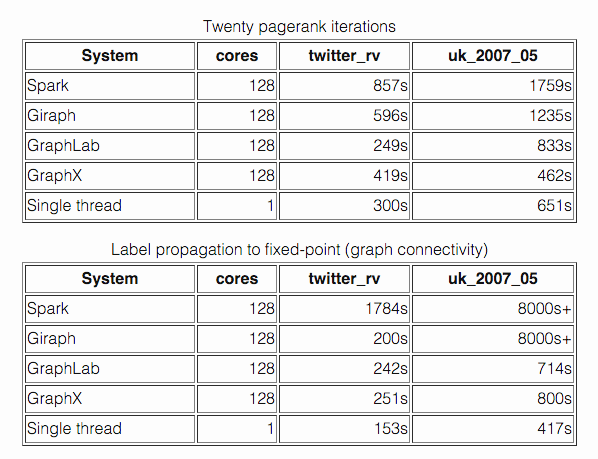
\includegraphics[width=0.80\textwidth]{images/pagerank.png}
\end{center}


\end{frame}



\begin{frame}
\frametitle{Takeaways}

\Large
\begin{changemargin}{1cm}

\begin{itemize}
\item    ``If you are going to use a big data system for yourself, see if it is faster than your laptop.''\\[1em]
\item    ``If you are going to build a big data system for others, see that it is faster than my laptop.''
\end{itemize}

\end{changemargin}
\end{frame}




\begin{frame}
\frametitle{Movie Hour, featuring NoSQL Bane}

Let's take a humorous look at cloud computing: James Mickens' session from Monitorama PDX 2014. 

\begin{center}
\url{https://vimeo.com/95066828}
\end{center}


\end{frame}

\end{document}

